%Remaining Anonymous when using the Bitcoin Protocol
\section{Introduction}
% Computer Society journal papers do something a tad strange with the very first
% section heading (almost always called "Introduction"). They place it ABOVE the
% main text! IEEEtran.cls currently does not do this for you.  However, You can
% achieve this effect by making LaTeX jump through some hoops via something
% like:
%
%\ifCLASSOPTIONcompsoc \noindent\raisebox{2\baselineskip}[0pt][0pt]%
%{\parbox{\columnwidth}{\section{Introduction}\label{sec:introduction}%
%\global\everypar=\everypar}}% \vspace{-1\baselineskip}\vspace{-\parskip}\par
%\else \section{Introduction}\label{sec:introduction}\par \fi
%
% Admittedly, this is a hack and may well be fragile, but seems to do the trick
% for me. Note the need to keep any \label that may be used right after \section
% in the above as the hack puts \section within a raised box.



% The very first letter is a 2 line initial drop letter followed by the rest of
% the first word in caps (small caps for compsoc).
% 
% form to use if the first word consists of a single letter:
% \IEEEPARstart{A}{demo} file is ....
% 
% form to use if you need the single drop letter followed by normal text
% (unknown if ever used by IEEE): \IEEEPARstart{A}{}demo file is ....
% 
% Some journals put the first two words in caps: \IEEEPARstart{T}{his demo} file
% is ....
% 
% Here we have the typical use of a "T" for an initial drop letter and "HIS" in
% caps to complete the first word.
%\IEEEPARstart{T}{his}

At 6:15 pm on the 3rd of January 2009, Satoshi Nakamoto (likely a pseudonym) created and announced a block of data known as the `Genesis Block' of the Bitcoin block chain~\cite{satoshi}. With this block, the first 50 units of the decentralized peer to peer currency, Bitcoin, were created\footnote{Strictly this isn't true, as due to a bug in the bitcoin client the first 50 bitcoins created cannot actually be spent.}. Since then, over ten million bitcoins have been generated.

The \textcite{euro-currency-schemes} (ECB) describes three different virtual currency schemes: closed currency schemes, unidirectional and bidirectional flow currency schemes.  Closed currency schemes involve currencies that cannot be converted to or from fiat currency\footnote{Fiat currency is a currency with a value given by government regulation such as the Great British Pound (GBP) or the United States Dollar (USD)}, an example of this would be `World of Warcraft gold'\footnote{\url{http://eu.battle.net/wow/en/shop/anti-gold/}} which cannot be bought using legal tender without violating the terms of service.  Unidirectional currency schemes include currencies like `Facebook Credits'\footnote{\url{https://www.facebook.com/credits/}} that can be purchased using legal tender but cannot be transfered to other users.  Finally, bidirectional currency schemes describe currency which can be converted to and from fiat currency, bitcoins are an example of this and are currently trading at \input{price}.

Bitcoin is distinct from other bidirectional digital currency schemes such as central banking and financial institutions or money transfer systems such as PayPal\cite{paypal} in that ``it is neither created nor administered by a single authority such as a central bank''\cite{why-interesting}, transactions are also irreversible are made pseudo-anonymously. The bitcoin protocol allows multiple different clients to connect, verify and disseminate transactions.  The reference bitcoin client, has received multiple releases\footnote{\url{http://bitcoin.org/en/version-history\#0.5.0}} and is now known as Bitcoin-Qt\cite{bitcoin-qt}. For the sake of brevity this paper will refer to Bitcoin-Qt Bitcoin client as the Bitcoin client.

TODO:
\begin{itemize} \item The need for bitcoin \item What this paper is about - The
    research on bitcoin, which has focussed on Anonymity, Economics and
    proposals for improvements \end{itemize}

\section{Background}
The core of any currency is to allow users to participate in transactions that result in transfer of value between the participants.  Such a system requires an element of trust or protocols that remove the need for trust between the participants.  If a user, Alice, wishes to send some value to Bob, Bob will need to know that Alice has the funds to send that transaction and has not sent or allocated that money to anyone else (a double spend). This problem is easily solvable using a physical transferable goods where the expense to duplicate or create more of a resource can be ensured to be more than the value of the item: for example creating counterfeit paper currency or creating a commodity like gold.  Although the issue of trust is somewhat negated with physical goods, they also encounter a separate issue - moving that value over distance.  This can be an expensive exercise as it requires both the expense of physically moving the good - particularly an issue with heavy gold bars - as well as the cost of securing it during transportation. While paper currencies solve these problems somewhat, with a trade-off of making duplication easier, a digital currency aims to recreate the difficulty in duplication, while taking advantage of the ease of transfer that digital information brings.

Up until relatively recently, discussions in scientific literature surrounding currency systems have assumed the necessity of some type of trusted central authority or authorities as part of the operation of the protocol.  These authorities usually maintain a record of transactions performed as well as minting and controlling the currency.  However, the relative success of Bitcoin has shown that this assumption is not necessarily the case and has increased discussion into decentralised currency - moving it from a topic of intellectual curiosity to one with more practical implications.

\subsection{Central Banking Authorities}

===================================================
===================================================
Services such as the UK ``Faster Payments Service''~\cite{guardian-fps}, or the ``Single Euro Payments Area'' (SEPA) payments initiative~\cite{SEPA} operate as a transfer protocol between users of trusted entities such as banks and other financial institutions.  While, payment processor systems and services, such as PayPal\footnote{\url{https://www.paypal.com/uk/webapps/mpp/transfer-money-online}}, Dwolla\footnote{\url{https://www.dwolla.com/individuals}} and Liberty Reserve\footnote{\url{http://web.archive.org/web/20130430103158/http://www.libertyreserve.com/}} operate on-top of existing currencies and, in exchange for money sent using SEPA or bank transfer, allow accounts to be credited with the equivalent value.  When a user requests a value transfer one account is debited while another is credited~\cite{paypal}.

While there are legal distinction between financial institutions and payment processors there is no significant technical distinction. These systems are effectively fully centralized, digital systems of exchange in which only the central authority or authorities control the minting of the currency or are able to create transactions.  An individual cannot create transactions and must rely on the central authority to make the transaction on their behalf.

These fully centralized systems have a simple design and implementation and often provide useful features such as insurance and interest.  However, during the operation of these systems some key disadvantages for the users have become apparent: the trusted entities have a legal responsibility to handle ``charge-backs'' or reverse transactions, the cost for this escrow service is placed on the customer as a transfer fee or to the merchant as a fine in the case of escrow failure. The second major disadvantage of these systems is that they are liable to be closed down due to legal pressure~\cite{lr-shutdown,lr-idictment}, or individual users' accounts can be frozen~\cite{mtgox-dwolla,vlad:mtgox-dwolla}.

In  systems where some trusted central authority exists, while it may be  reasonable to trust  some agent for the purpose of authenticating the  ownership of  value, that authority may act in a way outside of the  agents' control.  For example, if the server hosting the system is  compromised either through technical or legal means.

%uh oh this is duplicated...?
These fully centralized systems have a simple design and implementation however, there are some key issues that affect the users of the system - both merchants and customers - two of which are discussed here.  

The first issue is that the trusted entity has a legal responsibility to handle ``charge-backs'' or reverse transactions, the cost for this escrow service - in which the central authority acts as an arbiter in disputes - is placed on the customer as a transfer fee or to the merchant as a fine, or worse\cite{violin}.

The second major disadvantage of a centralized system is that it allows for  a single point of failure resulting in a lack of reliability from the  perspective of the user.  The central authority has complete control over the status of the users' account - that authority can freeze the funds of that account at their discretion according to their own terms of service, this can include pressure from legal authorities~\cite{mtgox-dwolla,vlad:mtgox-dwolla,wikileaks-paypal}.  Additionally, the central authority exists as an easier target for legal action, should that authority fail to freeze or track `problematic' accounts and this may result in a total shut down of that service~\cite{lr-shutdown,egold-shutdown,lr-idictment}. This report assumes that being resistant to attack from a third party, regardless of the good intentions of that party, is an advantageous feature of a currency.  It is not in the scope of this report to discuss the legal or ethical repercussions of such a system.

=============================================================

\subsection{Unique Token}
\textcite{netcash} discuss one solution, NetCash.  This protocol uses a unique token held by both the central authority and the owner of the coin. To create NetCash currency, the user and central authority agree on a unique token in exchange for some currency or resource. When that user wishes to transact value to another, they simply send the token to the other user.  A receiver can opt to trust the sender, thus remaining anonymous, or can trade-off anonymity for an assurance of validity from the central server.  To verify that the transaction is legitimate, receiving users send the token to the exchange, to be swapped for a new spendable token meaning the original token can no longer be spent. One issue with this protocol is the central authority cannot be independently verified, as such the central server may deny knowledge of a valid token, or allow multiple users to claim the same token and arbitrarily mint new tokens without a fee (either maliciously, due to being compromised or due to data loss).

\subsection{Blind-signed Chaumian e-Cash}
Proposed by \textcite{chaum}, the Chaum Token protocol, uses blind signatures. A user, Alice, creates a token $x$ and blinds it using function $c$.  A central authority will sign this blinded message using signing function $s$ in exchange for a fee, creating $s(c(x)$.  The authority then returns the blind signed message to Alice. Alice then removes the blind, leaving the signature $s(x)$ using $c^{-1}(s(c(x)))$.  These signed messages can now operate in a similar manner to tokens from the NetCash system: Alice can send $s(x)$ to Bob, who verifies the central authority's signature, and is now able to redeem this token with the central authority preventing Alice from sending the same token to another user.

The blinding protocol has the advantage that the central authority cannot discover the previous owner of a signed message when cashed by a payee because it is assumed that $c(x)$ cannot be derived from $s(x)$.  This protocol, however, maintains similar issues to NetCash: the central server may allow multiple users to claim the same token and arbitrarily mint new tokens without a fee (either maliciously, due to being compromised or due to data loss).

In both NetCash and Chaumian e-Cash the central server may accuse the original owner of the token of double spending the transaction.  Assuming Alice did not double spend the token, she now knows that the central server is dishonest, Bob on the other-hand cannot determine which of Alice or the central authority are being dishonest.

\subsection{B-Money digital signature chain}\label{digital-sig}
An alternative solution, B-Money proposed by~\textcite{b-money}, uses a chain of digital signatures where transaction messages are created using public key cryptography and the chain of digital signatures can be traced back to the original creation of the unit of value. In this system money is not sent per-se (only the transaction messages themselves are sent) but re-assigned.

``If Alice (owner of pseudonym $K_A$) wishes to transfer X units of money to Bob (owner of pseudonym $K_B$), she broadcasts the message ``I give X units of money to $K_B$'' signed by $K_A$'' for example see Figure~\ref{fig:chain-spend}.

This system presents the same problems as before regarding value distribution and potential double spending i.e. how does Bob know that Alice has the value to start with and how does Bob know that this value hasn't already been spent.  Figure~\ref{fig:chain-double-spend} gives an example of how a double spend might occur. \textcite{b-money} proposes two solutions to this problem: using a theoretical but impossible ``synchronous and unjammable anonymous broadcast channel'' or alternatively, to involve multiple trusted authorities that host a public copy of every transaction sent - if these peers attempt to show a differing view of history then fines can be levied from another peer.

Bob can download a copy of the transaction chain from one of these servers and verify that Alice was given some value from a chain of transactions leading back to the central authority where the value is assumed to be created and can subtract the total value of  Alice's spent transactions to determine if the transaction sent to Bob is valid.

\begin{figure}[t!]
    \centering
    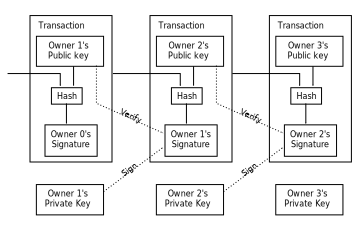
\includegraphics[width=\columnwidth]{img/Bitcoin_Transaction_Visual}
    \caption{A chain of digital signatures representing value transfer.
    (source \protect\cite{satoshi})}
    \label{fig:chain-spend}
\end{figure}

\begin{figure}[t!]
    \centering
    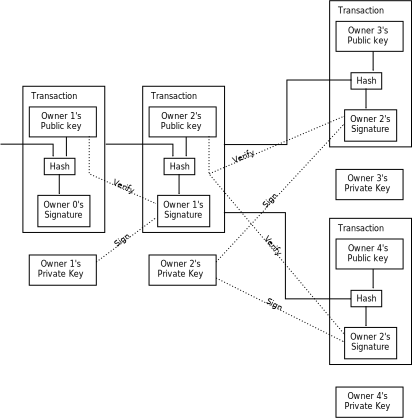
\includegraphics[width=\columnwidth]{img/Bitcoin_DoubleSpend_Visual}
    \caption{A chain of digital signatures representing value transfer with a double spend: Without some consensus system ``User 2'' is not prevented from sending the same value to both ``Owner 3'' and ``Owner 4''.
    (based on work from \protect\cite{satoshi})}
    \label{fig:chain-double-spend}
\end{figure}

The central authorities in this protocol also requires some degree of trust from the user that the authority is both benign and secure. For example, the central authorities could cooperate with, or more simply act as, a user attempting to achieve a double spend attack by showing different views to different users. Another reason that this currency was not adopted, was that a concrete implementation was never created and servers were never elected.

\section{The Bitcoin Protocol}
The Bitcoin protocol and client software~\textcite{satoshi} makes very few changes to the original b-money\cite{b-money} proposal. 

The Bitcoin protocol and client software provides a concrete implementation of an altered version of the original b-money proposal, with defined transaction syntax such as dynamic payment scripts and the concept of outputs that must be spent in their entirety.  The only significant novel deviation is that \textcite{satoshi} has substituted the ``synchronous and unjammable anonymous broadcast channel''~\cite{b-money} with a decentralized time stamp server that is used to ratify the order in which transactions occurred.  This allows for a dynamically changing set of transaction authorizing servers to achieve a consensus of valid transactions. Any user can, on receipt of a transaction, query the time stamp server and determine whether a transaction has been invalidated by a prior transaction. This key difference is likely the reason that Bitcoin took crypto-currencies from mathematical curiosity to a usable system for storage and transfer of value.

\subsection{Distributed Transaction Validation}
During the operation of the distributed time stamp server, the Bitcoin peer network, creates a chain of blocks of transactions, each referring to the previous by hash value. This is known as the Bitcoin block chain.  The transactions to be included in blocks in the chain are discovered when peers broadcast them into a peer discovery network that operates in a similar manner to a BitTorrent swarm\cite{swarm}.  Any user can contribute to this chain of blocks, but before another peer will relay it to others, it must meet a ``proof-of-work'' requirement: the double SHA-256 hash value of each block must not exceed a value determined by the current `difficulty'.  Because the SHA2 hashing function has been designed such that the value of an amount of data is unpredictable and evenly distributed in the range of the function, the only way for a participant to create data with a hash value below the difficulty limit is to repeatedly try different input data values\cite{btc-crypto}.  \textcite{satoshi} stated that ``The average work required is exponential in the number of zero bits required and can be verified by executing a single hash''. Transaction block data can be altered without changing the transaction semantics because the block format includes a `nonce' field for this purpose.

Because each block refers to the previous block, ``To modify a past block, an attacker would have to redo the proof-of-work of the block and all blocks after it''.  A peer in the Bitcoin network will accept a block if it has the highest total difficulty of any other block at that block height, shown in figure~\ref{ref:blockchain}, this allows the block chain to temporarily fork in the case that two blocks are created at the same time. The required difficulty of a valid block is re-calculated every 2016 blocks to ensure that block production takes the entire network an average of 10 minutes to solve.

\begin{figure}[t!]
    \centering
    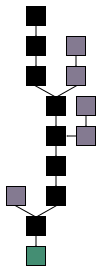
\includegraphics[height=\columnwidth]{img/Blockchain}
    \caption{A diagram showing invalid blocks (grey) being invalidated by a block chain with greater totaly difficulty (black). (based on work from theymos\protect\footnote{\url{http://theymos.com/}})}
    \label{fig:blockchain}
\end{figure}

As more blocks are created the more expensive it is for any group to alter the consensus reached by the peer network.  Because the proof of work system is computationally expensive an incentive, other than the increased certainty of any transaction a user has previously received will remain valid, is included.  While all the transactions included in a block must have at least the input value as output value, one transaction, the coinbase transaction, can be included with no input and an output dependent on the total number of blocks due to halve every 4 years. Currently this reward is 25 bitcoins. This reward is `paid' for by the consensual deflation of every participants' held bitcoin. This process also serves to solve the distribution problem of digital currencies.

\subsection{The Bitcoin block-chain is not strictly a consensus protocol}
\textcite{bitcoin-impossible} notes that, strictly, the Bitcoin proof of work block-chain is not a consensus scheme. In distributed consensus protocols, consensus is arrived at when some sufficient number of members of the group agree. This is impossible to achieve in a distributed system where this group is not known: agents are constantly joining and leaving the group in a way that prevents Sybil attacks. By declaring the Bitcoin group consensus definition as ``all the computing power in existence'' consensus is only achieved once more than half of the compute power in existence is used in the proof of work system. Therefore the Bitcoin system is only Sybil \emph{resistant}. The Bitcoin systems is also not fully decentralized, a set of core developers, now the Bitcoin Foundation, have some control of the protocol: two major disruptions to the network have been solved using manual intervention from this group: on 15 August 2010 an integer overflow was discovered in the Bitcoin protocol this vulnerability ``allows remote attackers to bypass intended economic restrictions and create many bitcoins via a crafted Bitcoin transaction.''~\cite{CVE-2010-5139}. The second, where the network segmented into clients with two differing consensus results~\cite{CVE-2013-3220,glitch-report,major-glitch}. Users of the network are still free to ignore the advice of this group.

\section{Related Work}
TODO: Related work, not covered in this report: Mentions of legal and economics papers eg. red-balloons \cite{red-balloons}.


\section{Anonymity}
As part of the Bitcoin protocol, all transactions must be broadcast publicly however, \textcite{satoshi} maintains that ``privacy can still be maintained by breaking the flow of information [...] by keeping public keys anonymous''.  Each Bitcoin address can be considered one pseudonym of many of the owner of the associated private key, because each person can own multiple Bitcoin addresses in a wallet. \textcite{satoshi} asserts that because of this disconnect between user and address it is difficult to associate a particular transaction with a particular user.


\subsection{Taint Analysis} \textcite{reid-anon}, considers the feasibility of maintaining this pseudo-anonymity in practise, by investigating the multiple input semantics of the Bitcoin transaction format. 

\textcite{reid-anon} argue that any key taking part in this process was in a single wallet, and thus owned by a single user. Therefore by combining the knowledge of how keys are grouped into wallets with knowledge from outside the protocol other inferences can be made, with the aim to determine the identity of the user behind the wallet, and thus any transactions made.

\textcite{reid-anon} aim to de-anonymize a user using two phases.  First to contract the publicly available, as published in the blockchain, ``transaction network'' to a ``user network'' by determining groups of addresses that appear to behave as part of a single wallet.  The second phase is to  link that group using publicly available ``Off-Network Information'' linking addresses to keys, eg by crawling the web for forum posts with including both user-names and addresses.

Multi-input transactions are used to distinguish the behavior of a group of keys from any other in the transaction network.  \textcite{eval-priv} add to this a further heuristic of ``Shadow Addresses'' to associate newly created addresses with users.

\subsubsection{Multi-input Transactions}
In the Bitcoin transaction format, if a user cannot fulfil the value of a transaction by spending a single previous output, the client will combine multiple inputs, or previous outputs, where the user has the ability to fulfil their spend conditions.  When combined the Bitcoin client must fulfil the spend conditions of all of the outputs, usually the conditions result in the requirement to sign the transaction with all of the participating private keys.  ``It is therefore straightforward to conclude that if these BTCs are (spendable) by different addresses, then the input addresses belong to the same user''\cite{eval-priv}.

[diagram of multi input transactions grouping wallets]

\subsubsection{``Shadow'' or Change addresses}
Because each previous oput must be redeemed in it's entirety, to support transactions of values smaller than the smallest output available to a wallet, the Bitcoin client automatically creates a new ``change address'' to send the remaining value to.  \cite{eval-priv} refers to this as a ``Shadow'' address.  The heuristic proposed, is that if money is sent to two or more addresses and only one has not been used before, that address is controlled by the user that created the transaction. A bug in the Bitcoin client was that it never randomized the outputs of the addresses and so this change address always appeared in a known location in the serialized transaction\cite{cve-ordered-trans}.

\begin{itemize} \item Briefly mentions mixers and ``repeatedly sending fractions
        of their Bitcoins to themselves using multiple (newly generated)
    public-keys'' Although that does not defeat taint analysis as these can be
assumed to be owned by the originating wallet until otherwise linked.  \item
    Change addresses, bug that lead to them being in the same position each
    time.  Androulaki et al, note that change addresses are clearly
    distinguishable by being the only newly generated address in the output of
    the transaction.  However it is recommended to newly generate a Bitcoin
    address for each receiving transaction.  \end{itemize}

\subsection{Taint Analysis Disruption}
\textcite{reid-anon} suggest repeatedly sending coins to new addresses. While this would gain anonymity under the reasoning of the paper, a new heuristic could be added to define that for addresses that have not yet been spent, and therefore linked with other addresses controlled by wallets known to be distinct, those addresses should inherit the status of the addresses that sent to it.

\subsubsection{Fully Trusted Mixing}
\textcite{eval-priv} note that it is possible to use a mixing service to fully disrupt their analysis.  A mixing service\footnote{\url{http://www.bitcoinlaundry.com/}} accepts Bitcoin transactions and automatically sends a new transaction otherwise unrelated with an equivalent ouput to a newly generated Bitcoin address.  These services often charge fees and require a significant amount of trust (bitcoin are totally in the control of the service before being returned).  The mixing service may also not have sufficient transaction traffic to be able to adequately hide the owner of bitcoin. Slight refinements on mixing services can be made by randomly adjusting the time that a transaction takes before being released or releasing multiple separate transactions into different newly generated addresses.

\subsubsection{ZeroCoin}
\textcite{zerocoin} propose a solution to the de-anonymization proposed in taint analysis, by defining new transaction types that take advantage of a zero knowledge proof (ZKP) that only proves knowledge of:

\begin{enumerate}
\item a Zerocoin in the block chain.
\item the actual serial number used to generate it.
\end{enumerate}

Formally, given all Zerocoins in the block chain ${C_1, C_2,\dots,C_N}$, prove knowledge of $C_i$ such that:

\begin{equation}
    (C_i = C_1) \vee (C_i=C_2) \vee \dots \vee (C_i=C_N)
\end{equation}

A ZKP for this statement is not efficient, as such Zerocoin uses a one-way public accumulator, with an efficient ZKP, that accumulates ${C_1, C_2,\dots,C_N}$ to produce some $A$, such that it's possible to prove knowledge of a witness s.t. $C \in inputs(A)$~\cite{one-way-accumulators}.

The function used, equation~\ref{eqn:zkp}, that provides this mathematical property under the strong RSA assumption was proposed by \textcite{strong-rsa}.

A Zerocoin $C_{i}$ is created using serial number $S$ in the group $Z(N)$ using a Peterson commitment, equation~\ref{eqn:zq-create}, repeated until $C_i$ is a prime.

\begin{equation}\label{eqn:zq-create}
C_{i}=g^Sh^r, C_i \in \mathbb(P)
\end{equation}

An accumulator $A$ can be created from the asserted Zerocoins.  Adding to the accumulator is trivial, $A' = A*u^{C_i}$.

\begin{subequations}
    \begin{align}\label{eqn:zkp}
        N &= p \cdot q, u \in QR_{N}(u\neq1)\\
        A &= u^{C_1, C_2,\dots,C_N}\\
        w_i &=  u^{C_1, C_2,\cdots C_{i-1}, C_{i+1}, \dots ,C_N}
    \end{align}
\end{subequations}

Where N is the product of two permanently private prime numbers (These primes are generated once, multiplied then are permanently destroyed).

The Zero-knowledge proof, proves that $u^{C_i} \cdot w_i = A$. $w_i$ is now defined as the new accumulator. Unfortunately, this proof requires a 40KiB Double Discrete Logarithm proof, and the modification of all Bitcoin clients on the network which strictly is a new currency and no longer Bitcoin, but another incompatible block chain currency.

\subsubsection{In-Protocol Mixing}
In his forum post, ``I taint rich!'', Bitcoin developer Gregory (gmaxwell) Maxwell describes a process to disrupt ``brain-dead automated (taint) analysis''.  Because the conditions of a set of previous outputs can be fulfilled partially, multiple users can cooperate to create a single transaction that causes their public keys to appear linked in a single wallet to taint analysis, without revealing their private keys to the group.  As such the claim made by \textcite{satoshi}, and key assumption made by \textcite{reid-anon}, that ``Some linking is still unavoidable with multi-input transactions, which necessarily reveal that their inputs were owned by the same user'' is wrong.

While in the example described it is clear how the addresses are truly linked in the user graph, due to the cooperation being performed on a public forum, the same address used on the input and output and the fact that that address is the vanity address, ``1gmaxw''. The complexity of this process means it is not well used.

[diagram showing this specific transaction]

For a serious attempt to disrupt taint analysis the taint disrupting transaction must have the following properties:  Each output must be to an address that has not been used previously. There must be an equal number of bitcoin sent to each output. The transaction must not be traceable to a network address.  The communication during cooperation must not be intercepted. The communication must not be shown to have taken place.  At this point, from a view of the block chain, the two wallets appear linked, under the multi-transaction heuristic and change address heuristic. From the view of the cooperating peers, however, it is clear the true owner of the output keys as such this process must take place repeatedly between many different peers.

[diagram showing generic mixing transaction]

\begin{itemize} \item Using the Tor hidden service \item Some sort of central or
        distributed registration system for peers \item A peer may connect to
            any other peer, each peer creates a new address, they both determine
            an equal amount of bitcoin to send. And create a multi-input
            transaction from both users, split equally into the new addresses.
\item Assuming that the ownership of originating addresses was known publicly
the ownership of the two new addresses is now 50/50.  \item Diagram \item Repeat
the process
\end{itemize}

TODO: describe and compare with everyone mix, vs pairwise mixing. Esp. re: DoS.

\section{Conclusion}
While it is clear that the de-anonymization techniques will be no-longer be applicable once the anonymization techniques discussed in this report become widely used by users of the Bitcoin system, it is not obvious that they will be applicable even to existing network data. Any adversary well versed in the protocol would have been able to avoid de-anonymization even before the Bitcoin client\cite{bitcoin-qt} added support for multi-input and output transactions and the dangers of address re-use were widely publicized because these techniques were already available when interacting with the network directly with command line tools.


\section{Future Work}
This report discusses only a proposal for a novel anonymization system, an obvious avenue for further work would be to design, create and test a concrete implementation. Other avenues for further work would to be to investigate design changes and improvements to the existing Bitcoin system: would using multi-cast for transaction distribution enhance the protocol; create tools to allow easy data-mining of block-chain data using ideas from the Linked Open Data or Semantic Web communities.

%\section{Alternative Post-Bitcoin Digital Currencies}

%\subsection{Bitcoin-like protocols}
%TODO: What makes a protocol different to Bitcoin? Why is this important?

%\subsubsection{Upgrades and Maintenance}
%TODO: Bitcoin foundation, not strictly devoid of authority.

%\subsection{Improvements and Differences}
%TODO: Litecoin, Feathercoin. Why not Ripple?

%\begin{itemize} \item What is a forking change?  \item What improvements are
%possible \item The hash power voting system \end{itemize}


% An example of a floating figure using the graphicx package.  Note that \label
    % must occur AFTER (or within) \caption.  For figures, \caption should occur
    % after the \includegraphics.  Note that IEEEtran v1.7 and later has special
    % internal code that is designed to preserve the operation of \label within
    % \caption even when the captionsoff option is in effect. However, because
    % of
% issues like this, it may be the safest practice to put all your \label just
    % after \caption rather than within \caption{}.
%
% Reminder: the "draftcls" or "draftclsnofoot", not "draft", class option should
    % be used if it is desired that the figures are to be displayed while in
    % draft mode.
%
%\begin{figure}[!t] \centering \includegraphics[width=2.5in]{myfigure} where an
    %.eps filename suffix will be assumed under latex, and a .pdf suffix will be
    %assumed for pdflatex; or what has been declared via
    %\DeclareGraphicsExtensions.  \caption{Simulation Results.} \label{fig_sim}
    %\end{figure}

% Note that IEEE typically puts floats only at the top, even when this results
    % in a large percentage of a column being occupied by floats.  However, the
    % Computer Society has been known to put floats at the bottom.


% An example of a double column floating figure using two subfigures.  (The
    % subfig.sty package must be loaded for this to work.) The subfigure \label
    % commands are set within each subfloat command, and the \label for the
    % overall figure must come after \caption.  \hfil is used as a separator to
    % get equal spacing.  Watch out that the combined width of all the
    % subfigures on a line
% do not exceed the text width or a line break will occur.
%
%\begin{figure*}[!t] \centering \subfloat[Case
    %I]{\includegraphics[width=2.5in]{box}% \label{fig_first_case}} \hfil
    %\subfloat[Case II]{\includegraphics[width=2.5in]{box}%
    %\label{fig_second_case}} \caption{Simulation results.} \label{fig_sim}
    %\end{figure*}
%
% Note that often IEEE papers with subfigures do not employ subfigure captions
    % (using the optional argument to \subfloat[]), but instead will
    % reference/describe all of them (a), (b), etc., within the main caption.


% An example of a floating table. Note that, for IEEE style tables, the \caption
    % command should come BEFORE the table. Table text will default to
    % \footnotesize as IEEE normally uses this smaller font for tables.  The
    % \label must come after \caption as always.
%
%\begin{table}[!t] % increase table row spacing, adjust to taste
    %\renewcommand{\arraystretch}{1.3} if using array.sty, it might be a good
    %idea to tweak the value of \extrarowheight as needed to properly center the
    %text within the cells \caption{An Example of a Table} \label{table_example}
    %\centering % Some packages, such as MDW tools, offer better commands for
%making tables % than the plain LaTeX2e tabular which is used here.
    %\begin{tabular}{|c||c|} \hline One & Two\\ \hline Three & Four\\ \hline
    %\end{tabular} \end{table}


% Note that IEEE does not put floats in the very first column - or typically
    % anywhere on the first page for that matter. Also, in-text middle ("here")
    % positioning is not used. Most IEEE journals use top floats exclusively.
    % However, Computer Society journals sometimes do use bottom floats - bear
    % this in mind when choosing appropriate optional arguments for the
    % figure/table
% environments.  Note that, LaTeX2e, unlike IEEE journals, places footnotes
    % above bottom floats. This can be corrected via the \fnbelowfloat command
    % of the stfloats package.